\documentclass[tikz,border=4pt]{standalone}

\usepackage{amsmath}
\usepackage{amssymb}
\usetikzlibrary{arrows.meta,calc}

\definecolor{viablue}{HTML}{6CA2C6}
\definecolor{axisgray}{HTML}{555555}
\definecolor{guidegray}{HTML}{999999}

\begin{document}
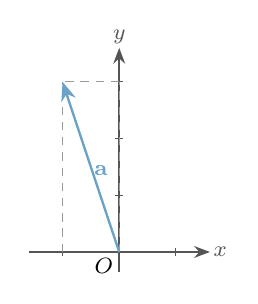
\begin{tikzpicture}[
    scale=0.72,
    >=Stealth,
    axis/.style={->, semithick, axisgray},
    guide/.style={dash pattern=on 3pt off 2.5pt, guidegray},
    vec/.style={-{Stealth[length=2.4mm,width=1.9mm]}, line width=0.85pt, viablue},
    tick/.style={axisgray, thin},
    lbl/.style={font=\footnotesize, inner sep=1pt}
  ]
  % Axes
  \draw[axis] (-1.6,0) -- (1.6,0) node[right, lbl] {$x$};
  \draw[axis] (0,-0.35) -- (0,3.6) node[above, lbl] {$y$};
  \node[lbl, below left=1pt] at (0,0) {$O$};

  % Axis ticks (no numeric labels)
  \draw[tick] (-1,-0.07) -- (-1,0.07);
  \draw[tick] (1,-0.07) -- (1,0.07);
  \draw[tick] (-0.07,1) -- (0.07,1);
  \draw[tick] (-0.07,2) -- (0.07,2);
  \draw[tick] (-0.07,3) -- (0.07,3);

  % Component guides
  \draw[guide] (0,0) -- (0,3);
  \draw[guide] (0,3) -- (-1,3);
  \draw[guide] (-1,0) -- (-1,3);

  % Vector
  \draw[vec] (0,0) -- (-1,3);
  \node[lbl, text=viablue] at ($(0,0)!0.46!(-1,3) + (0.14, 0.06)$) {$\mathbf{a}$};
\end{tikzpicture}
\end{document}
